
\documentclass[12pt]{article}

\usepackage{sbc-template}

\usepackage{hyperref}
\hypersetup{
    colorlinks=true,
    linkcolor=blue,
    filecolor=magenta,      
    urlcolor= blue,
    bookmarks=true,
    pdfpagemode=FullScreen,
}


\usepackage{url}

\usepackage{graphicx,url}
\usepackage{amsmath}
\usepackage[brazil]{babel}   
\usepackage[utf8]{inputenc}  
\usepackage{units}
\usepackage{fancyhdr}

\usepackage{indentfirst}
\usepackage[inline]{enumitem}
\pagestyle{fancy}

\fancyhead[L]{ }
\fancyhead[R]{ }

%\chead{\begin{picture}(3,3) \put(-230,-15) {\includegraphics%[width=16cm, height=2.8cm, keepaspectratio=false]{logoSIRC.png}} \end{picture}}
\renewcommand{\headrulewidth}{0pt}
\sloppy
\begin{document} 


\title{Relatório técnico sobre o avanço da pandemia causada pelo vírus SARS-CoV-2 na cidade de Dourados - MS:\\ reavaliação do cenário do município e entorno}

\author{Fernando Ferraz Ribeiro\inst{1}, Marco Aurélio Boselli\inst{2},\\ Everaldo Freitas Guedes\inst{3}, Fernanda Vasques Ferreira\inst{4}}


\address{Universidade Federal da Bahia -- Faculdade de Arquitetura -- LCAD
  (UFBA)\\
  Salvador, BA -- Brasil
\nextinstitute
  Universidade Federal de Uberlândia  -- Instituto de Física (UFU)\\
  Uberlândia, MG -- Brasil 
\nextinstitute
  Bacharel em Estatística, Doutor e Mestre em \\Modelagem Computacional Aplicada à Tecnologia Industrial\\
  Salvador, BA -- Brasil
\nextinstitute
  Universidade Federal do Oeste da Bahia (UFOB)\\
  Santa Maria da Vitória, BA -- Brasil
  \email{fernando.ribeiro@ufba.br, maboselli@gmail.br, }\email{efgestatistico@gmail.com,
  fernanda.jornalista82@gmail.com}
}


\maketitle

\begin{abstract}

This report presents a reevaluation of the study on the progress of the pandemic caused by the SARS-CoV2 virus in the municipality of Dourados - MS. Originally published with data collected until 06/23/2020, this second evaluation round updates the scenario, compiling the information made available until 07/07/2020, addresses the need for improvements in the availability of data on the pandemic and reassessment the errors and successes of the predictions made using the DELPHI model previously presented. At the end, the conclusions are reported.

\end{abstract}
     
\begin{resumo}

Este relatório apresenta uma reavaliação do estudo sobre o avanço da pandemia causada pelo vírus SARS-CoV2 no município de Dourados - MS. Publicado originalmente com dados coletados até o dia 23/06/2020, esta segunda rodada de avaliação atualiza o cenário, compilando as informações disponibilizadas até o dia 08/07/2020,  trata da necessidade de aprimoramentos na disponibilização dos dados sobre a pandemia e reavalia os erros e acertos das predições realizadas através do modelo DELPHI apresentadas anteriormente. Ao final as conclusões são reportadas.

\end{resumo}


\section{Introdução}

\begin{figure}[!htb]
  \centering
  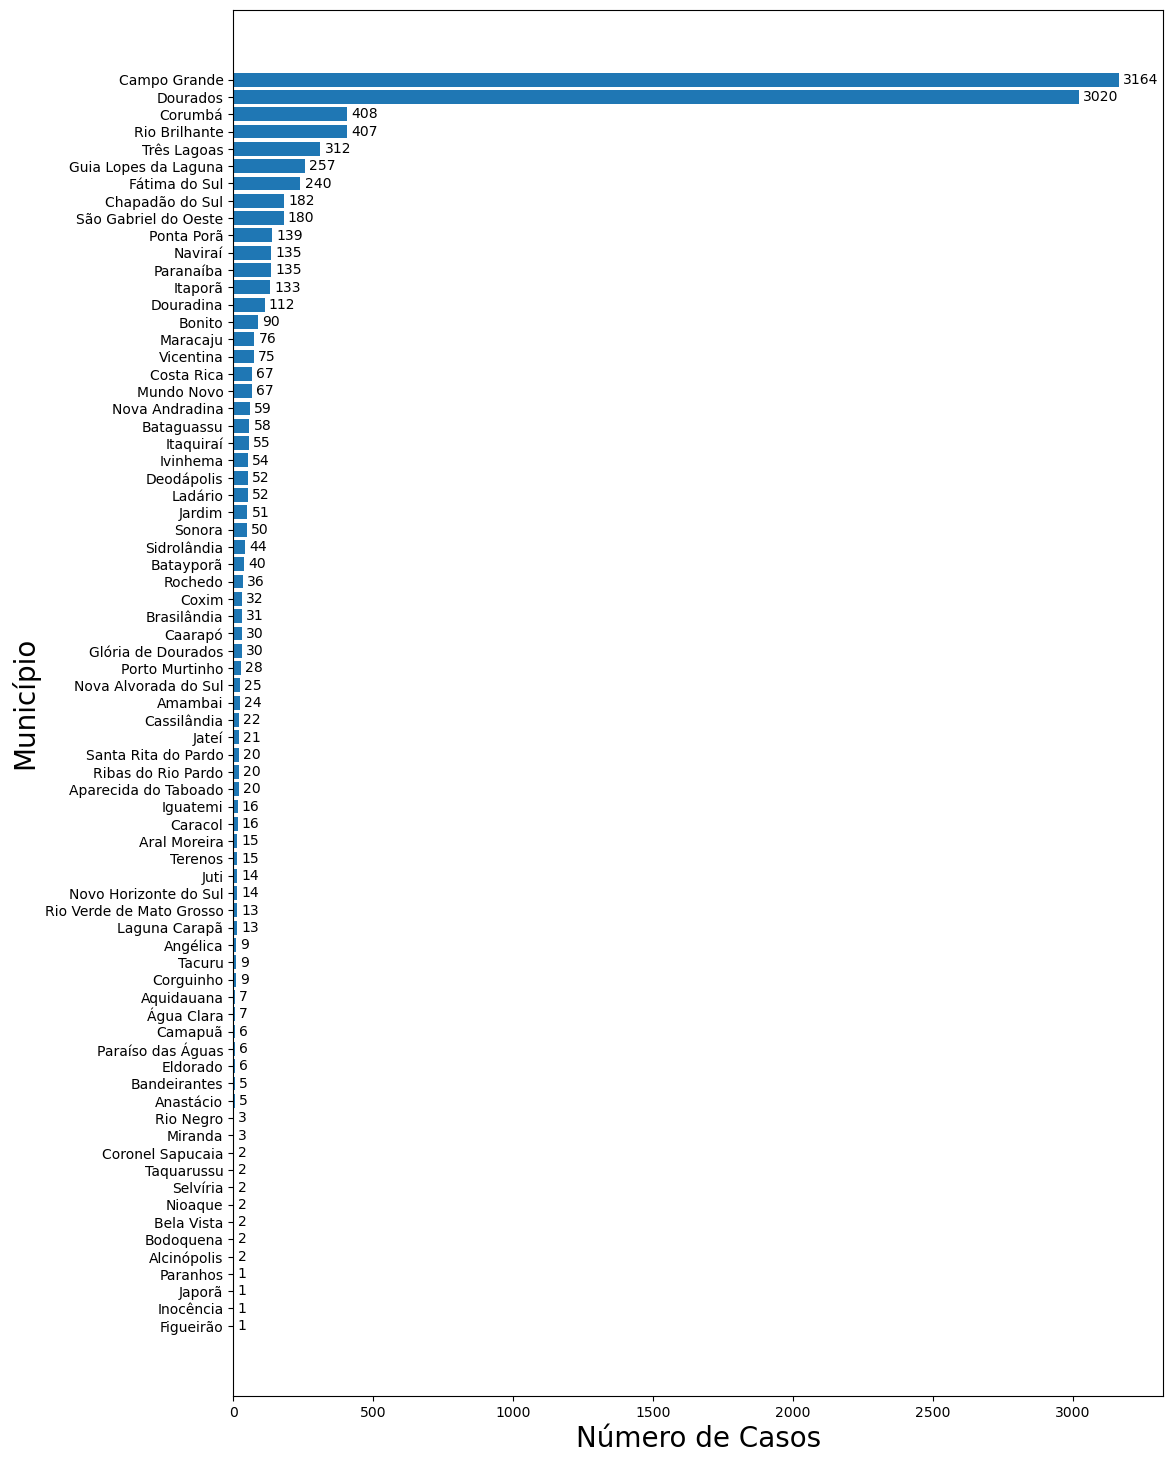
\includegraphics[width=1\textwidth]{figs/casos_por_municipio.png}
  \caption{Número de casos diagnosticados por município (MS) extraídos do boletim epidemiológico do dia 07/07/2020}
  \label{fig:casosMuni}
  \end{figure}

Na época da primeira avaliação do cenário da pandemia na região de Dourados -MS realizada por este grupo de pesquisa, a universidade \textit{Johns Hopkins University}, apontava que o número de infectados pelo vírus SARS-CoV-2 no mundo rondava a casa dos 9 milhões (em 23/06/2020). Nesta segunda rodada, pouco mais de 14 dias depois, a mesma instituição aponta que a casa dos 12 milhões foi ultrapassada (09/07/2020).

\begin{figure}[!htb]
  \centering
  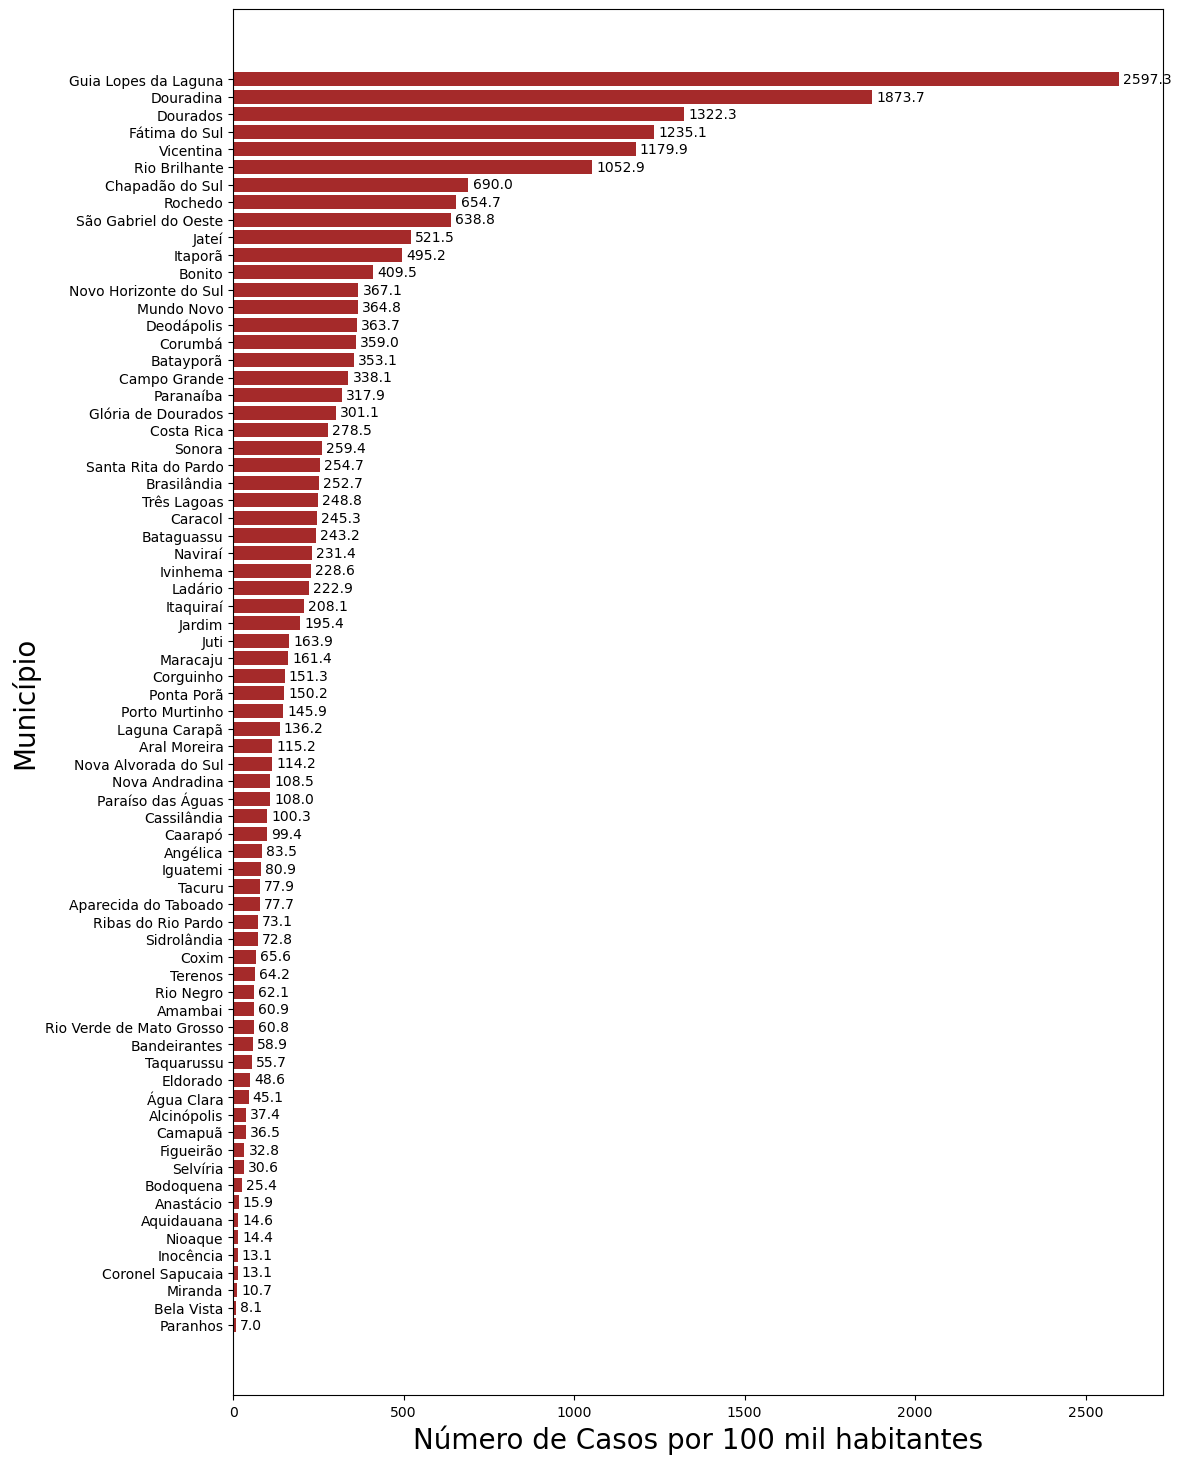
\includegraphics[width=1\textwidth]{figs/casos_100_mil_por_municipio.png}
  \caption{Número de casos por 100 mil habitantes em cada município (MS) extraídos do boletim epidemiológico do dia 07/07/2020}
  \label{fig:casosMuni100k}
  \end{figure}


Este relatório reavalia o cenário com dados disponibilizados até o dia 07/07/2020, data que corresponde com o final do período analisado pelo modelo preditivo na publicação anterior. Novas previsões são realizadas, com base nos dados coletados até o dia 08/07/2020. Assim como no resto do mundo, o avanço da pandemia nesta região justifica o acompanhamento e reavaliação dos dados.

\section{Metodologia}\label{sec:met}

A metodologia segue muitas das balizas utilizadas no relatório anterior. A análise de dados é refeita e comparada com o que foi observado anteriormente, tendo por fonte de dados o mesmo repositório utilizado anteriormente \textbf{CORONAVÍRUS BRASIL}\cite{minsaude}.

Em seguida, uma avaliação da quantidade de testes realizados e de como a divulgação e disponibilização destes dados são feitas. Sugestões, críticas e elogios sobre a formatação destes dados não são direcionadas unicamente ao município de Dourados, mas se estende para os demais municípios do estado e do país.

\section{Evolução do cenário}\label{sec:dados}

Na última avaliação, o município de Dourados contabilizava 1.964 casos notificados. Passadas duas semanas, conforme Figura~\ref{fig:casosMuni}, o total alcançou 3.095, um acréscimo em torno de 40\% em um curto período de tempo. Em números totais, o município de Campo Grande ocupa agora a primeira posição do estado. Já em termos relativos, Dourados subiu da quinta posição para a terceira. Já a capital do estado, subiu da vigésima terceira para a décima quinta, como pode ser observado na figura~\ref{fig:casosMuni100k}.

\begin{figure}[!htb]
  \centering
  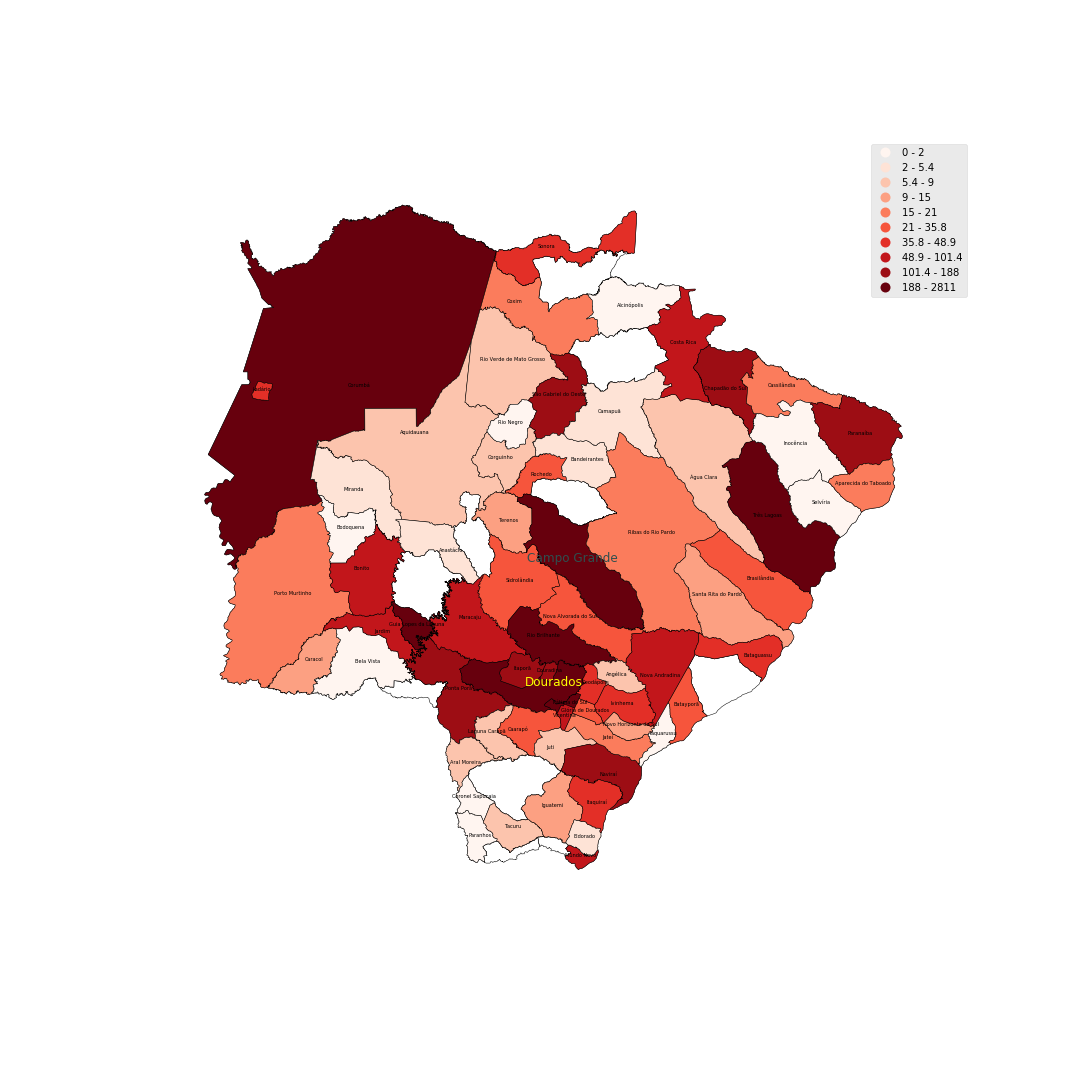
\includegraphics[width=1\textwidth]{figs/mapa_casos_registrados.png}
  \caption{Mapa de casos diagnosticados por município (MS) extraídos do boletim epidemiológico do dia 07/07/2020}
  \label{fig:mapaCasos}
  \end{figure}


O município de Guia Lopes da Laguna, em primeiro lugar na quantidade de casos por 100 mil habitantes nos dois momentos, apresentou um pequeno acréscimo de casos durante o período decorrido (de 254 para 257 casos). Douradina, em segundo lugar, subiu de 94 para 113 casos no mesmo intervalo de tempo. 

\subsection{Dados Geoespaciais}\label{ssec:geo}

Em termos geográficos, a centralidade do município de Dourados na distribuição dos casos permanece. Tanto do ponto de vista absoluto, conforme Figura~\ref{fig:mapaCasos}, quanto do relativo, expresso na Figura~\ref{fig:mapa100K}.

\begin{figure}[!htb]
  \centering
  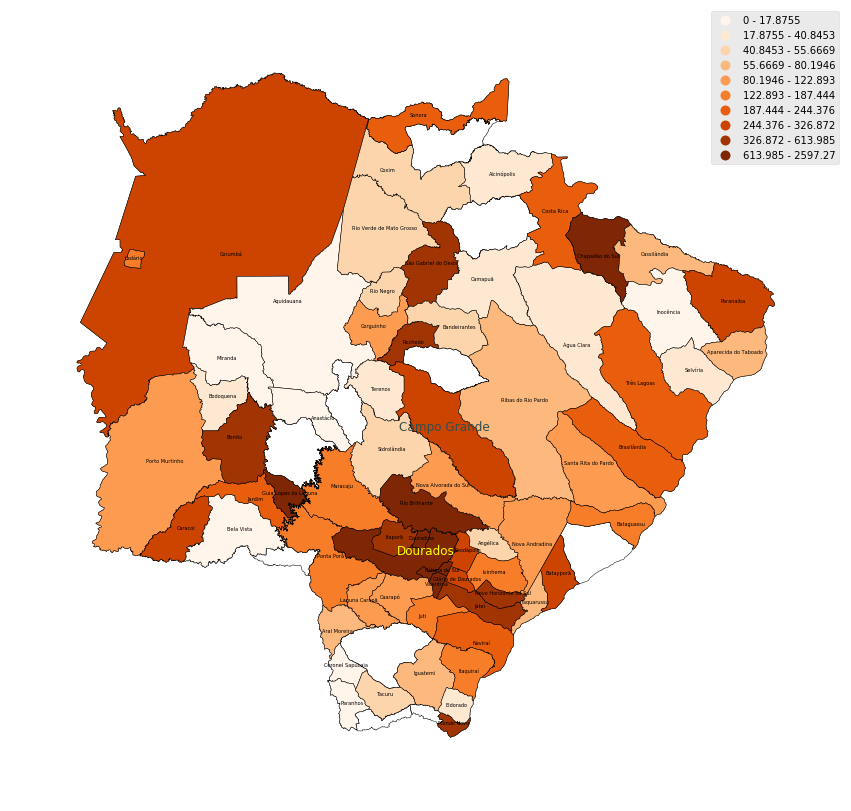
\includegraphics[width=.8\textwidth]{figs/mapa_casos_100_mil.png}
  \caption{Número de casos diagnosticados por 100 mil habitantes em cada município (MS) extraídos do boletim epidemiológico do dia 07/07/2020}
  \label{fig:mapa100K}
  \end{figure}

Muito embora a proporção entre o número de casos do estado e os números apresentados tanto no município, quanto no município e seu entorno imediato e expandido tenha diminuído, questiona-se se isso se deve primordialmente à diminuição do ritmo de propagação na cidade (abordado na seção~\ref{ssec:curvas}), a uma flutuação nas dinâmicas de testagem (seção \ref{ssec:pubDados}) ou à disseminação da pandemia no estado de forma mais homogénea.

O espalhamento do vírus no estado pode ser constatado pela comparação entre os mapas apresentados neste estudo e suas versões apresentadas na edição anterior. Não é um caso particular do estado do Mato Grosso do Sul, este comportamento pode ser visto em praticamente todo o território nacional.

\begin{figure}[!htb]
  \centering
  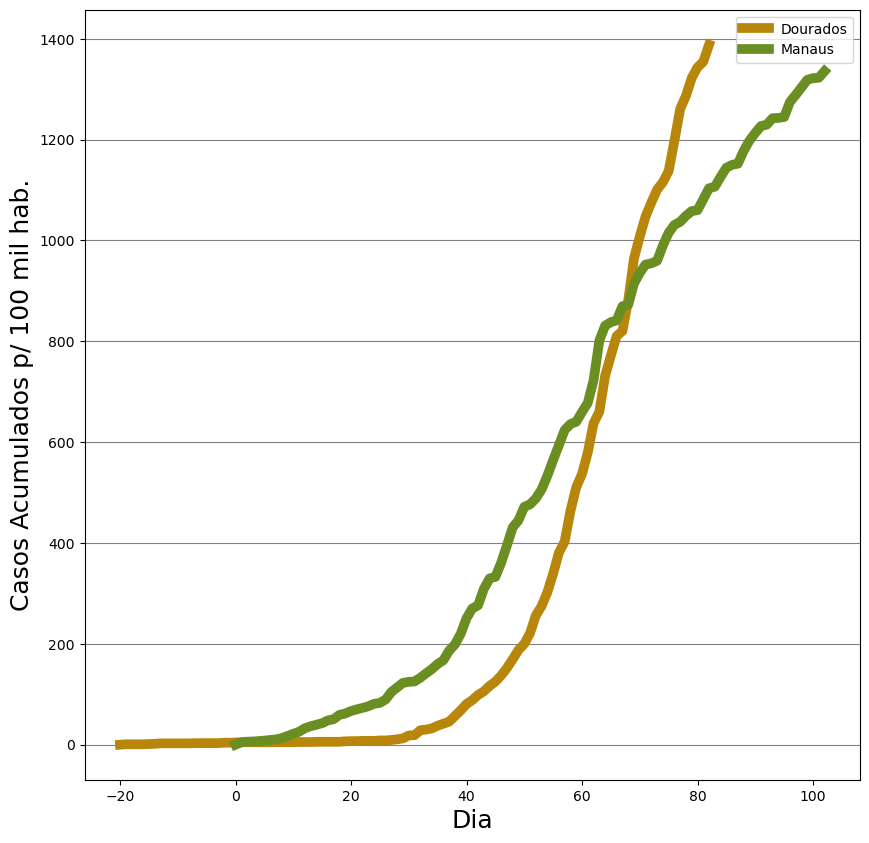
\includegraphics[width=.5\textwidth]{figs/Dourados_Manaus_casos.png}
  \caption{Curva do número de casos diagnosticados por 100 mil habitantes. Comparativo entre Dourados (MS) e Manaus (AM)}
  \label{fig:curva100K}
  \end{figure}

Na Figura~\ref{fig:mapa100K}, Dourados e municípios do entorno aparecem em grande destaque. Embora outros municípios do estado estejam representados na mesma faixa de cor, apenas a região de Dourados e entorno conecta múltiplos municípios na classificação mais alta de casos por 100 mil habitantes.

\begin{figure}[!htb]
  \centering
  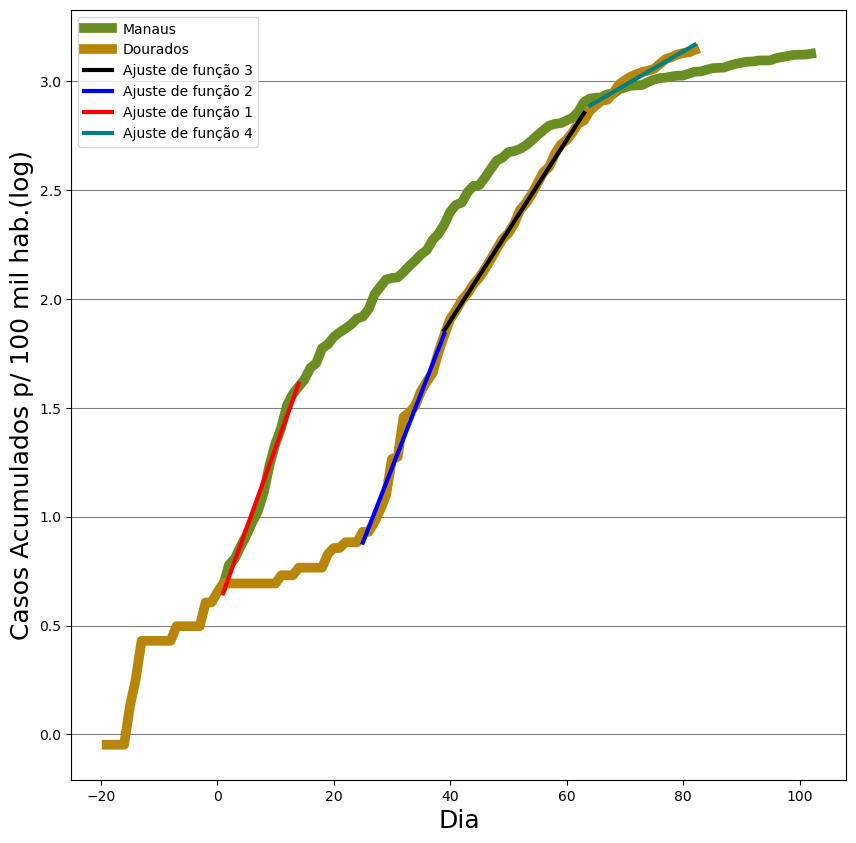
\includegraphics[width=.5\textwidth]{figs/Dourados_Manaus_casos_log.png}
  \caption{Curva do número de casos diagnosticados por 100 mil habitantes. Comparativo entre Dourados (MS) e Manaus (AM) em escala logarítmica (eixo y)}
  \label{fig:curva100KLog}
  \end{figure}

\subsection{Curva da evolução de casos}\label{ssec:curvas}

Na Figura~\ref{fig:curva100K}, vemos que o número de casos por 100 mil habitantes em Dourados ultrapassou o número registrado em Manaus. Embora a velocidade de crescimento registrada na Figura~\ref{fig:curva100KLog}, ainda nota-se um crescimento exponencial bem descrito pelo trecho do gráfico marcado com a legenda "ajuste de função 4".

É preciso reforçar a noção de que a comparação da evolução do número de casos em localidades diferentes tem sérias limitações. A intenção ao fazê-la, em consonância com outros estudos internacionais, é ter uma ideia mais precisa do quão rápida está se dando a evolução do cenário. A cidade de Manaus é aqui utilizada como um caso modelo, no qual o pico já foi atingido. O colapso sofrido pelo sistema de saúde na capital do Amazonas acontece quando o limite deste sistema é atingido. Se os sistemas de saúde das duas cidades tivessem características equivalentes, o colapso também já teria atingido a cidade objeto deste estudo.

\subsection{Históricos de testagem e publicação das informações}\label{ssec:pubDados}

As curvas de casos acumulados, apresentadas na subseção~\ref{ssec:curvas}, não devem ser o único critério de avaliação do curso da pandemia em um determinado lugar. A simples divulgação do número de testes positivos aferidos em um dia pelos laboratórios de análises não é um indicador suficiente para diversas conclusões.

\begin{figure}[!htb]
  \centering
  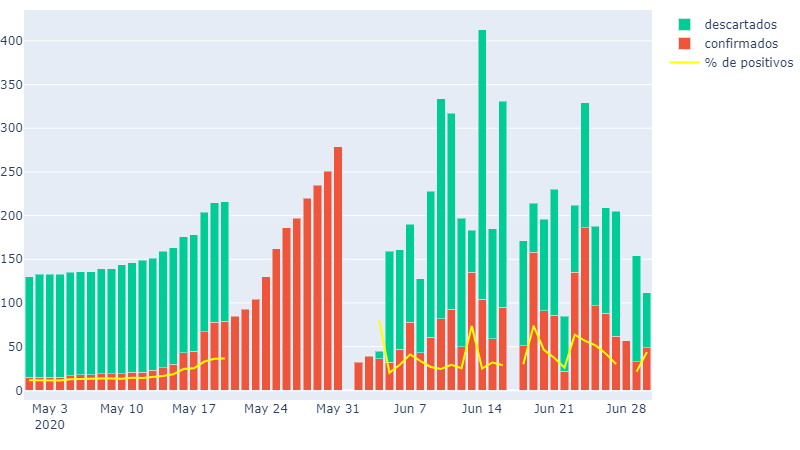
\includegraphics[width=.75\textwidth]{figs/casos_conf_desc.png}
  \caption{Reconstrução do histórico de casos confirmados e descartados com base nos boletins epidemiológicos da prefeitura}
  \label{fig:histTeste}
  \end{figure}

Existem exames diferentes, cujos resultados devem ser avaliados com distintos critérios: um tipo detecta a presença do vírus nas vias respiratórias, indicando que a doença está ativa no organismo do indivíduo e que este é um possível transmissor da Covid-19; o outro tipo detecta anticorpos específicos para o SARS-CoV-2, indicando que o paciente testado teve contato com o patógeno e, possivelmente, já não apresenta um quadro que ainda possibilita a infecção de outras pessoas.

\begin{figure}[!htb]
  \centering
  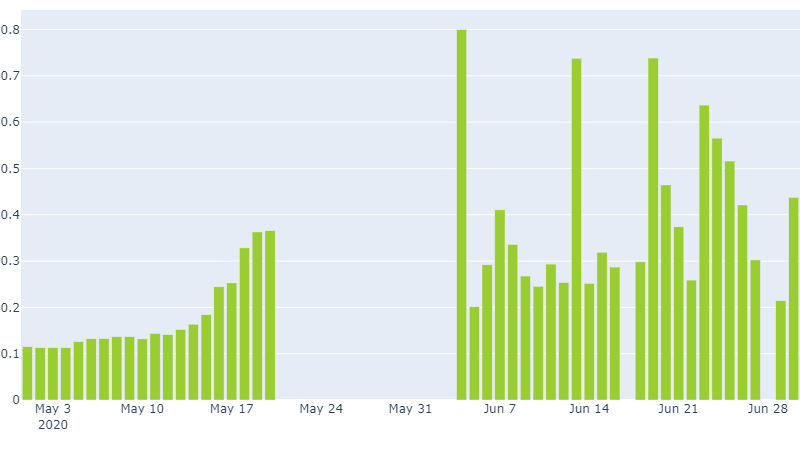
\includegraphics[width=.75\textwidth]{figs/taxa_positivo.png}
  \caption{Taxa de casos positivos com base nos boletins epidemiológicos da prefeitura}
  \label{fig:positTaxa}
  \end{figure}


Além do tipo de exame e da quantidade de casos positivos, é preciso saber quantos casos foram descartados de um mesmo conjunto de exames enviados para testes. Se o número de testes totais é maior, provavelmente o número de infectados aumentará. Se um gestor diminui a quantidade de testes, pode gerar a falsa impressão de que o quadro da cidade melhorou, simplesmente porque o número total de infectados caiu.

A prefeitura de Dourados vem divulgando boletins informativos que apresentam o número de casos confirmados e descartados todos os dias. Esses boletins podem ser encontrados em formato de imagem digital no portal do município. Os dados destes boletins entre os meses de maio e junho foram compilados durante esta pesquisa, na tentativa de recriar o histórico de testagem para que este também pudesse ser analisado.

A equipe reconhece o empenho da prefeitura em divulgar os números de testes confirmados e descartados para o novo coronavírus, mas dificuldades foram encontradas em aferir estes números. Na Figura~\ref{fig:histTeste} vemos os dados que conseguimos recuperar: do dia 1º ao dia 20 de maio foram encontradas as informações sobre o total de positivos e de descartados. Entre o dia 21 e 31 de maio, bem como nos dias 2 e 3 de junho, apenas o número de testes positivos foi encontrado. Nos dias 1º e 17 de junho, não foram encontrados os boletins informativos.

\begin{figure}[!htb]
  \centering
  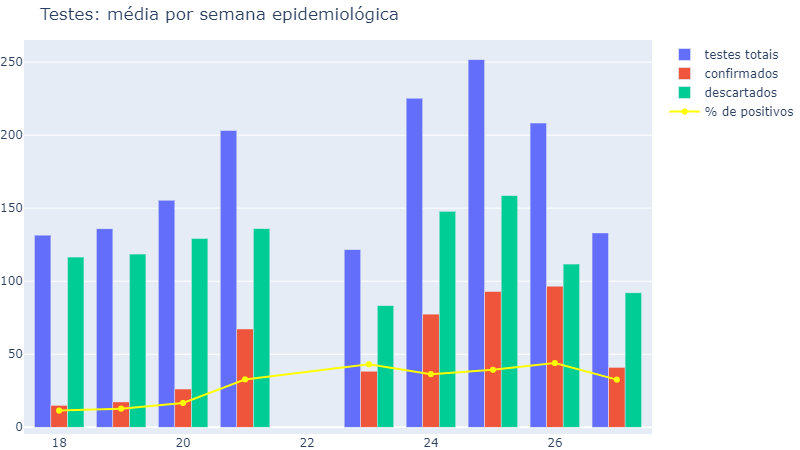
\includegraphics[width=.75\textwidth]{figs/media_cof_desc.png}
  \caption{Média de casos totais, confirmados e descartados com base nos boletins epidemiológicos da prefeitura}
  \label{fig:medTeste}
  \end{figure}

Apenas nos dias em que os números de casos confirmados e descartados são encontrados, pode-se calcular a taxa de casos positivos deste período de exames. A figura~\ref{fig:positTaxa} mostra esta taxa para os dias em que foi possível calcular, seguindo a fórmula \( \nicefrac{P}{P+D}\), onde \(P\) representa o número de casos positivos e \(D\) o número de casos totais. Note-se que em alguns, principalmente no mês de junho, esses valores ficam acima da margem de falso negativo dos testes, chegando a atingir \(0.8\) no dia 04/07/2020, indicando que 80\% dos casos são aferidos como positivo.

Taxas de positivo muito elevadas podem indicar um nível de testagem baixo em relação ao tamanho da população, ou que se está testando principalmente os indivíduos com quadros mais graves.

A Figura~\ref{fig:medTeste} apresenta uma interpretação do histórico do número de testes por semana epidemiológica. Devido à dificuldade de se reconstituir o histórico completo de testes, adotou-se uma média semanal, excluindo assim os dias em que a taxa de positivos não pôde ser calculada. Na semana epidemiológica 25 chegamos ao máximo de 252 testes em média por dia, na semana seguinte a média cai para 208 testes. Para a semana 27, vale ressaltar que apenas os dois primeiros dias foram englobados no período de testes recuperado nesta pesquisa, e isso pode afetar a média, visto que o número de resultados reportados tem apresentado variação entre os dias da semana.

Na semana 26 também encontramos a maior média semanal da taxa de positivos da série, em torno de 44\% do total. O governo do estado do Mato Grosso do Sul tem disponibilizado juntamente com seus boletins epidemiológicos \cite{BoletinsMS} uma tabela de dados chamada de ``microdados". Um conjunto de informações relevantes e organizadas sobre os pacientes testados como positivos apresenta o tipo de testes, a cidade de residência e a cidade onde o exame foi feito e um resumo das condições físicas e de saúde do paciente. Apresentados de maneira ética, sem que os pacientes possam ser identificados pelas informações postas, o relatório omite, no entanto os casos onde o resultado do exame apontou negativo para o vírus SARS-CoV-2.


\section{Modelo Preditivo}\label{sec:predit}

O relatório técnico de 24/06/2020 apresentou o modelo DELPHI \cite{delphi}, com suas características, defeitos e possibilidades de ajuda em estudos e entendimento de epidemias. Segue aqui uma avaliação da evolução dos casos e óbitos após 14 dias decorridos do primeiro estudo. 

\begin{figure}[!htb]
  \centering
  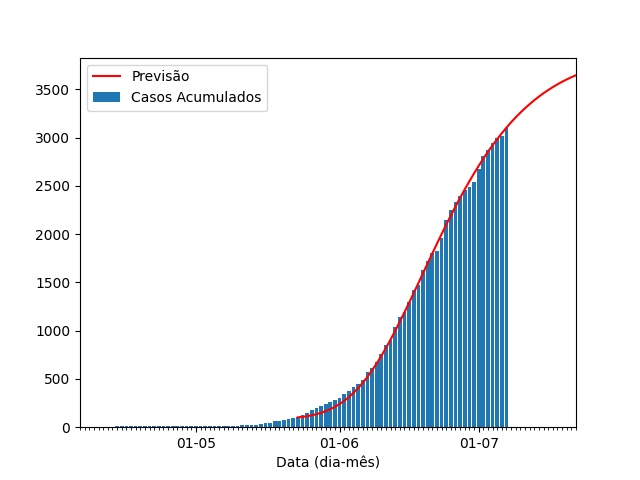
\includegraphics[width = 8cm]{figs/Fig_Brasil_MS_Dourados_casos_20200708.jpg}
  \caption{As barras azuis são número total de casos acumulados segundo o Ministério da Saúde para a cidade de Dourados - MS, e em vermelho a curva de previsão do modelo DELPHI para 14 dias.}
  \label{proj_casos}
 \end{figure}
 
Os dados analisados foram coletados do Portal Coronavírus do Ministério da Saúde \cite{minsaude} no dia 08/07/2020 e são relativos à divulgação dos dados do dia anterior. A predição do modelo é mostrado na Figura \ref{proj_casos} para os casos acumulados para o município de Dourados MS e na Figura \ref{proj_obitos} para o número de óbitos acumulados.  

\begin{figure}[!htb]
  \centering
  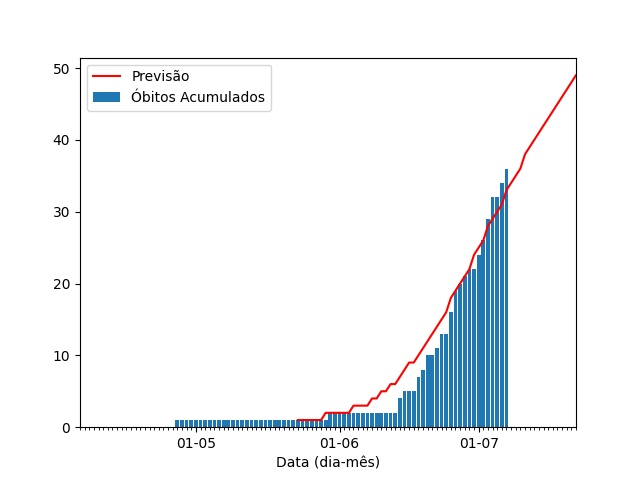
\includegraphics[width=8cm]{figs/Fig_Brasil_MS_Dourados_obitos_20200708.jpg}
  \caption{Gráfico de óbitos. Barras azuis são casos acumulados e curva vermelha previsão do modelo DELPHI para 14 dias.}
  \label{proj_obitos}
 \end{figure}

Na Figura \ref{proj_casos} vemos que o regime ainda é de crescimento de casos, e o platô da curva ainda não aparece nesta previsão. A predição do modelo é mostrado na Figura \ref{proj_casos} para os casos acumulados para o município de Dourados MS e na Figura \ref{proj_obitos} para o número de óbitos acumulados.

Parte dos parâmetros do modelo é feito com peso maior nos óbitos acumulados, dados mostrados na Figura \ref{proj_obitos}. Nesta nova previsão, assim como na anterior do dia 24/06/2020, a curva de predição tem indicativo de crescimento. E, novamente, a previsão para os últimos 6 dias está abaixo dos números reais (barras azuis). Isto é um indicativo que para os próximos dias o crescimento de óbitos estará acima desta previsão.   

\section{Conclusão}\label{conc}

O modelo preditivo aplicado aos dados de Dourados revela que o município ainda se encontra numa fase de crescimento da pandemia. Recomenda-se o uso ou o reforço, se for o caso, de medidas sanitárias recomendadas pelas autoridades em saúde, principalmente aquelas que mostraram sucesso na contenção da pandemia que acometeu China, Coreia e Europa de forma bastante intensa. Até o momento o que se mostrou mais eficiente foi o isolamento social numa situação de transmissão sustentada. A testagem em massa e o rastreio dos contatos dos casos registrados também se mostrou eficiente.

A apresentação dos dados e o número de testes não é um problema exclusivo de uma cidade, região ou estado do Brasil. A pesquisa reconhece o empenho da prefeitura em divulgar estas informações em seus boletins. Contudo, procuramos chamar a atenção para a diferença entra a divulgação e a disponibilização. Um arquivo de imagem com as informações sobre a pandemia é uma maneira de se divulgar dados para a população, mas seria importante disponibilizar as informações em outros formatos para que pesquisadores, divulgadores científicos, educadores e a imprensa possam acessar de forma mais fácil, não o dado de um determinado dia, mas os históricos das informações sobre esta crise sanitária. Recomendamos que as informações da planilha de ``microdados'' do estado do Mato Grosso do Sul passe a divulgar também o histórico dos casos negativos. Também deve-se pensar em uma forma sistemática de divulgar o número de leitos, vagos e ocupados, de enfermaria e UTI, públicos e privados por cidade e região do estado.


A situação da pandemia se agrava no estado, e o município de Dourados, bem como seu entorno imediato, ainda representam um ponto focal importante neste contexto. Este relatório tem por objetivo apresentar elementos deste cenário para as autoridades responsáveis pela definição das politicas públicas de enfrentamento da crise, com a intenção de colaborar com a luta diárias por momentos melhores.

\bibliographystyle{sbc}
\bibliography{modelo.bib}

\end{document}
